
This paper demonstrates how CNN and ensemble models can be used to classify multiple cardiac abnormalities using 12-lead ECG-recordings. The cross-validated results show that the ensemble model, using features from 12 leads, outperforms the other nine models on the development dataset from PhysioNet/CinC Challenge 2020. F1, F2, G2 and the PhysioNet/CinC Challenge Score were used to score the models. The 12-lead ensemble model was significantly better than all other models, measured on all four metrics.

The winner of PhysioNet/CinC Challenge 2020 reported a mean  cross-validated PhysioNet/CinC Challenge Score of $0.533\pm0.046$ SD \cite{natarajan_wide_nodate}, which was slightly better than the best score achieved in this study: $0.512\pm 0.006$. It is important to bear in mind that the cross-validated scores achieved on the development set, in this study, should be compared with caution to the reported scores on the PhysioNet/CinC Challenge 2020 hidden test set from other studies \cite{natarajan_wide_nodate,singstad_convolutional_nodate}. Even if some papers demonstrated good agreement between their cross-validated results, on the development set, and the results achieved on the hidden test set \cite{natarajan_wide_nodate}, the organizer reported that high-performing algorithms exhibited significant drops ($\approx 10\%$) in performance on the hidden test data \cite{alday_classification_2020}.

Surprisingly, the CNNs with the lowest complexity performed best compared to the rest of the CNNs. The Encoder model was significantly better in terms of F1, F2 and G2-score (figure \ref{fig:crossval_score}a-c), but closely followed by FCN and FCN $||$ Gender\&Age when looking at the PhysioNet/CinC Challenge Score (Figure \ref{fig:crossval_score}d). Nevertheless, it is stated in \cite{singstad_convolutional_nodate} that the Encoder performed worse than FCN $||$ Gender\&Age, Encoder $||$ Gender\&Age, Encoder $||$ FCN + rule-based model and Encoder $||$ FCN $||$ Gender\&Age + rule-based model on a subset of the hidden test set. This observation emphasizes that one should be careful when comparing cross-validated scores with scores achieved on the hidden test set.

The FCN $||$ Encoder and the FCN $||$ Encoder $||$ Gender\&Age appeared to be unaffected by adding the rule-based model. No significant differences can be seen for any of the scoring methods in figure \ref{fig:crossval_score}. A possible explanation for this might be that the rule-based model always agreed with the CNN-model and thus did not change the prediction. Another possible explanation for this is that the rule-based algorithms failed to analyze the ECG and then did not make any prediction. One should keep in mind that these rule-based algorithms were really simple and therefore these results should be interpreted with caution.

Another surprising aspect was that the ensemble model, using features from 2 leads, performed significantly better than all CNN models, using all 12 leads, on the PhysioNet Challenge Score (figure \ref{fig:crossval_score}d). However, it should be mentioned that the Encoder performed equally well on the F1, F2 and G2-score as seen in figure \ref{fig:crossval_score}a-c.

A possible limitation in this study is that the ECGs were not filtered before feeding them into the model or before extracting features with the ECG-featurizer. Some of the ECGs had a lot of noise, like the ECG in figure \ref{fig:noisy_leadII}. Further studies are needed to determine if a filtered ECG signal would improve the performance of the models used in this study.

\begin{figure}[!hbp]
    \centering
    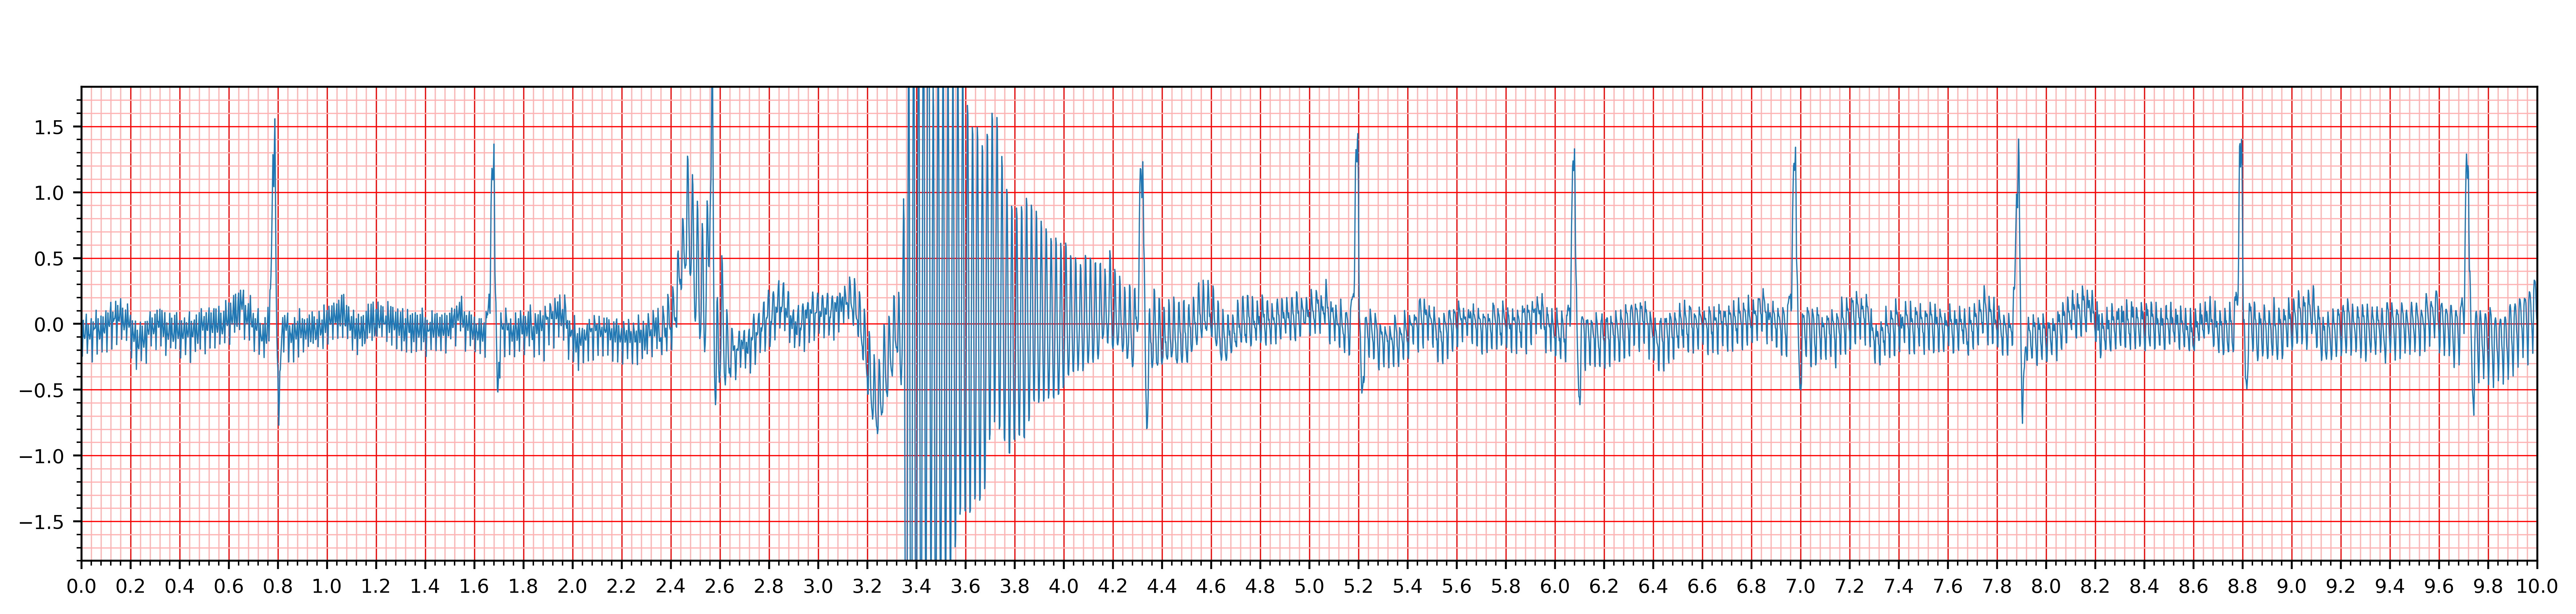
\includegraphics[width=.90\textwidth]{Figures/noisy_leadII.png}
    \caption{The figure shows an example, from the development set, of a noisy ECG-signal from lead II}
    \label{fig:noisy_leadII}
\end{figure}

This research has demonstrated two slightly different methods of using explainable AI with ECG classifiers. The prediction made by the ensemble model is based on the extracted ECG features using the ECG-featurizer and therefore the explanation, by LIME, are related and limited to these features. On the other hand, the prediction made by the CNN models is based on $12 \times 5000$ samples giving LIME more features to use in its explanation.




Even if the ensemble model only used a few features ($112$) compared to the CNN models ($12 \times 5000$), the explanation provided for the ensemble model seems to be more understandable in this case. In figure \ref{fig:explainability_rand_12} the most important explanation for the AF prediction  was the standard deviation of the heart rate calculated from the R-peaks. This explanation can be supported by physiological knowledge.

The explanation of the ECG time series has shown to have some potential \cite{strodthoff_deep_2020,zhang_interpretable_2020}. However, in this study, there is hard to see any patterns from the three segments highlighted by the recurrent explainer in figure \ref{fig:expl_cnn}. In future research, the recurrent  explainer should be programmed to return more of the features that were used in the prediction to see any patterns.

A general limitation with LIME is that it is built on a weak mathematical foundation compared to for example the SHAP library \cite{lundberg_unified_2017} (Shapley values). 
In future investigations, it should be considered to use a different approach like the SHAP library to explain the predictions of the classifiers. 


Despite the results showing that explainable AI methods can be used to explain the classification of ECGs, there is still a lot of work to be done in this field. It is important to make sure that the explanations are valuable for potential end-users (doctors/cardiologists). In future investigations, it also might be possible for the developer to use the explanation to identify possible weaknesses of the classification model by looking at the explanations. Our findings emphasize the need to continue to develop explainable models for time series classifiers like the ECG models demonstrated in this study. 